\begin{figure}[tbp]
  \centering
  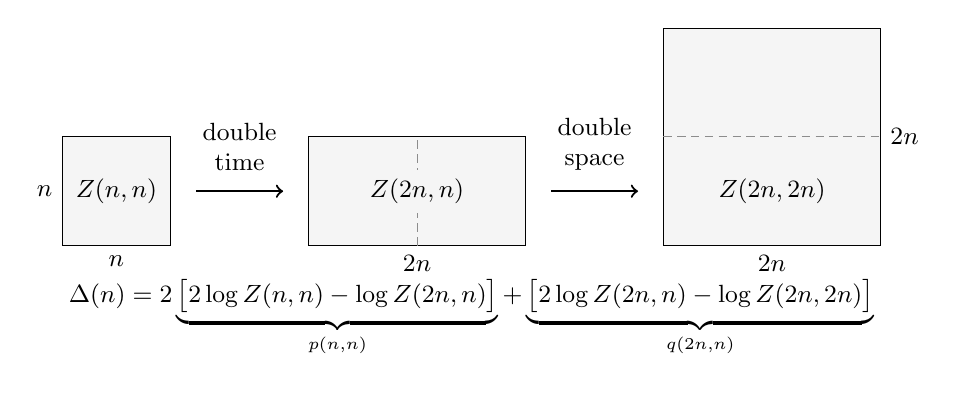
\begin{tikzpicture}[x=0.92cm,y=0.92cm,font=\small]
    \draw[fill=black!4] (0,0) rectangle (1.5,1.5);
    \node at (0.75,0.75) {$Z(n,n)$};
    \node[below] at (0.75,0) {$n$};
    \node[left] at (0,0.75) {$n$};

    \draw[->,thick] (1.85,0.75) -- (3.05,0.75);
    \node[align=center,above] at (2.45,0.9) {double\\time};

    \draw[fill=black!4] (3.4,0) rectangle (6.4,1.5);
    \draw[densely dashed,black!45] (4.9,0) -- (4.9,1.5);
    \node[fill=black!4] at (4.9,0.75) {$Z(2n,n)$};
    \node[below] at (4.9,0) {$2n$};

    \draw[->,thick] (6.75,0.75) -- (7.95,0.75);
    \node[align=center,above] at (7.35,0.9) {double\\space};

    \draw[fill=black!4] (8.3,0) rectangle (11.3,3);
    \draw[densely dashed,black!45] (8.3,1.5) -- (11.3,1.5);
    \node at (9.8,0.75) {$Z(2n,2n)$};
    \node[below] at (9.8,0) {$2n$};
    \node[right] at (11.3,1.5) {$2n$};

    \node at (5.65,-1.0)
      {$\displaystyle
        \Delta(n)=2\underbrace{\bigl[2\log Z(n,n)-\log Z(2n,n)\bigr]}_{p(n,n)}
          +\underbrace{\bigl[2\log Z(2n,n)-\log Z(2n,2n)\bigr]}_{q(2n,n)}$};
  \end{tikzpicture}\par\medskip
  \caption{The two coordinate directions enter the square-box test.
  Every rectangle has periodic boundary conditions; the dashed lines
  mark its dimensions, not cuts that make the pieces independent.
  The second doubling starts from the enlarged rectangle.
  The displayed identity is exact, with the fixed coupling suppressed.}
  \label{fig:rectangle-doubling}
\end{figure}
